\documentclass{amsart}
\usepackage{graphicx}
\graphicspath{{./}}
\usepackage{hyperref}
\usepackage{csvsimple}
\usepackage{longtable}
\usepackage{lscape}
\usepackage{epigraph}
\title{May 22 2021:  My Health Condition Degenerates Further} 
\author{Zulfikar Moinuddin Ahmed}
\date{\today}
\begin{document}
\maketitle

\section{The Invasion and Destruction of my meta continues}

The White Supremacist Butcher Bill Gates, who began an assault into my eyes and meta more than six months ago as reciprocation for my R\& D and sale of my Medium Frequency Alpha Strategy that D. E. Shaw \& Co. is trading because the abominable, low, illiterate ignorant and stupid Bill Gates is under the mistaken notion that massive violation of my Natural Rights are permitted by the United States since he has various special privileges.  I, American, have constantly sought to get involvement of US Senate and US Supreme Court and other agencies of US Government to use US Defense Forces to bomb and kill Bill Gates.  

US Government has thus far not done the right thing and have not killed Bill Gates yet.

I woke up quite sick and without any employment contract or any other Bill Gates had been using power against me.  I will hold United States responsible for these egregious violations of my Natural Rights and their penalty I will set to \$1 trillion.  They have not performed adequately, for US Declaration of Independence leaves no ambiguity about the fundamental purpose of their ability to seem important in the world and get paid from taxes of other people.  They must secure Natural Rights of Americans, including mine.  

The corruption of America seems at epidemic levels at the moment.

\section{How Did the Great Genius Zulf Exploit Bernoulli Variables to Get Precise Estimates for Ethnicity Effects on Morals?}

I never liked coin tossing ever since I was young.  I never thought learning about calculating probabilities of number of coins doing this or that would ever amount to anything serious, and never got interested in gambling either.  It was only after I already had a job at Fixed Income Derivative Research as a quant in 1995 that I thought that probabilistic models are serious.  In recent years I have been studying history of probability theory more seriously.  

What I thought was going on, that Pascal and Fermat were French Aristocrats who were actually in the business of gambling were interested in games of chance for this reason, and by chance scientific inference become identified with all manner of coin tossing afterward.

The actual history is not very far from this.  In eighteenth century people were attempting to produce scientific inference from binomial model.

In any case, some centuries of practice in proving all sorts of theorems for flipping biased coins led to quite a bit of sharp understanding about Bernoulli two-valued random variables.

So I decided yesterday that there might be some advantages in interpretability if we take advantage of the analysis of universal human values with World Values Survey questions Q7-Q17 which are binary, for inference on the effects of ethnicity on these.

\section{Proposal For a New Method to Determine True Probability $p$}

Suppose we have a sequence of $N$ independent Bernoulli random variables with the same distribution.  Let us order them as $X_1,\dots, X_N$.  

We are interested in determining the true parameter $p$ for probability $P(X_j=1)=p$.  

We do not know $p$, but we are able to sample the $X_1, \dots, X_N$.  We pick these from Nature.

We propose the following.  We take $K<< N$ such as $K=10$.  Then we take the sequences
$Y_1 = (X_1, \dots, X_{10})$ and 
\[
Y_r = (X_{1+r},\dots, X_{10+r})
\]

Then we sweep through the full sequence and obtain the best $p$ that fits empirical frequencies to the formula
\[
Q(k) = \choose{10}{k}p^k (1-p)^{10-k}
\]
The benefit of this method will be that we are simultaneously fitting $2^{10}$ numbers.  This is a bit too high.  We can reduce to $K=6$.  Let's see, that's $64$ differing numbers.  Might do with $K=5$, and 32 numbers.

Anyway, we expect that fitting 32 numbers will give us a better estimate for $p$ than just taking the empirical frequency at the end and appealing to Weak Law of Large numbers.

\section{Working Code}

\begin{verbatim}
library(nloptr)

# We have 11 genuine bona fide Bernoulli random
# variables from Nature here and not from
# all manner of disreputable institutions
# from Nevada and Atlantic City and so on
# and it is a great opportunity to actually
# do Bernoulli analysis for inference for
# true parameter

# Diatribe:  the true parameter of a Bernoulli
# random variable from Nature is not a "biased coin"
# I cannot stand Science and Man's great ambitions 
# regarding the truth of Nature reduced to sordid
# business of gambling and all sorts of unsavory 
# and depressing characters without meaning in their
# lives who have their savings taken away by these
# predatory charlatans.  
# We will be saving the reputation of binary random
# variables from gambling houses.

chvars<-c("Q7","Q8","Q9","Q10", "Q11",
          "Q12", "Q13", "Q14", "Q15", "Q16", "Q17")


zulf.bernoulli.p.est<-function( x, K){
  N <- length(x)
  xd<-matrix(0, nrow = N-K, ncol = K)
  for ( r in 1:(N-K)){
    xd[r,] <- t(x[r:(r+(K-1)),1])
  }
  xdtbl<-table( data.frame(xd))
  
  objfun<-function( p ){
    v <- 0
    for (k in 1:2^K){
      for (r in 1:K) {
        theoretical <- log(choose(K,r)) + 
                      r*log(p) + (K-r)*log(1-p)
        
        empirical <- count_r_heads( xd )
        v <- v + ( theoretical - empirical )^2
      }
    }
    return (sqrt(v))
  }
  x0<-0.5
  res<-nloptr(x0, eval_f=objfun, eval_grad_f = NULL, 
         lb = 0.0, ub = 1.0)
  res$solution
}



K <- 3
x<-na.omit(polv[,"Q7"])
print(dim(x))
N <- dim(x)[1]
xd<-matrix(0, nrow = N-K, ncol = K)
for ( r in 1:(N-K)){
  xd[r,] <- t(x[r:(r+(K-1)),1])
}
#xdtbl<-table( data.frame(xd))

count_r_heads<-function( xd, r, K){
  vc <- 0
  nr <- nrow( xd )
  for (s in 1:nr){
   tfreq <- table( xd[s,])
   if ( tfreq[1] == r ){
     vc <- vc + 1
   }
  }
  vc/2^K
}
  
objfun<-function( p){
  v <- 0
  for (k in 1:2^K){
    for (r in 1:K) {
      theoretical <- log(choose(K,r)) + 
        r*log(p) + (K-r)*log(1-p)
      
      empirical <- log(count_r_heads( xd, r, K))
      v <- v + ( theoretical - empirical )^2
    }
  }
  out<-sqrt(v)
  print(out)
  out
}
x0<-c(0.5)

nopts <- list("algorithm"="NLOPT_LN_COBYLA",
             "xtol_rel"=1.0e-8)

res<-nloptr(x0, eval_f=objfun, eval_grad_f = NULL, 
            lb = 0.0, ub = 1.0, opts = nopts )

res$solution

\end{verbatim}

\section{Announcement}

Ladies and Gentlemen,

With the great new innovation of estimating Bernoulli parameter p from data, the World will never be the same again.  Once again, the great scientific Genius Zulfikar Moinuddin Ahmed produces even more precise method of seeking the SECRETS OF NATURE.

HAHAHAHAHAHAHAHAHA
HAHAHAHAHAHAHA
HAHAHAHAHAHAHAHAHA
HAHAHAHAHAHAHAHA

And soon all of Nature's Secrets shall be OURS!!  No no no, let Victoria have her secrets.  We are reputable gentlemen here.  Now now Victoria, run along.  We are interested in NATURE's Secrets not yours.

Thanks,
ZULFIKAR MOINUDDIN AHMED


\section{Test to Show that My Method Vastly Improves Upon Frequency Count}

Frequency count does converge by Weak Law to the true Bernoulli parameter $p$.  But the convergence might be quite slow.

For Q7 I have $N=19077$; these are Bernoulli 1/2 answers.

I let $x$ be the first 500 values.  Then I use my technique to estimate $p$.  I obtain $p_{Zulf}=0.7267$.  In contrast I obtain $p_{Freq} = 0.904$.  The difference is 
\[
|p_{Zulf} - p_{Freq}| = 0.1773
\]
That is not a small error, and our ordinary intuition for $N=500$ points would demand better accuracy.

Let us consider the full frequency to confirm $p_{Zulf}$ as a better estimate.  The full sample gives frequency $p_{Freq;N=19077}=0.811$.

Let's accept $p_* = p_{Freq;N=19077}$ as 'truth' for now.

Then we get
\[
|p_{Zulf} - p_*| = 0.08474
\]
and
\[
|p_{Freq} - p_*| = 0.0916
\]
My estimate then is getting to 'truth' by 0.0069.

Not only did my method get closer to truth, but 0.7\% is nothing small in $N=500$ for accuracy of a frequency.

\section{Improved Code and Improvement with $N=1500$ sample by Zulf Estimate}

For sample size of $N=1500$, we considered the frequency estimate of a much larger $N=19077$ elements as the truth.  We also have $p_{Zulf}$ and $p_{Samp}$ for our estimates on $N=1500$ data.  Our results:

\[
|p_{Zulf} - p_{True}| = 0.0384
\]
and
\[
| p_{Samp} - p_{Truth} | = 0.0519
\]
Our improvement is 
\[
\Delta = 0.0135
\]
That is a very significant improvement for $N=1500$.

\begin{verbatim}
library(nloptr)
require(compiler)
enableJIT(3)

# We have 11 genuine bona fide Bernoulli random
# variables from Nature here and not from
# all manner of disreputable institutions
# from Nevada and Atlantic City and so on
# and it is a great opportunity to actually
# do Bernoulli analysis for inference for
# true parameter

# Diatribe:  the true parameter of a Bernoulli
# random variable from Nature is not a "biased coin"
# I cannot stand Science and Man's great ambitions 
# regarding the truth of Nature reduced to sordid
# business of gambling and all sorts of unsavory 
# and depressing characters without meaning in their
# lives who have their savings taken away by these
# predatory charlatans.  
# We will be saving the reputation of binary random
# variables from gambling houses.

chvars<-c("Q7","Q8","Q9","Q10", "Q11",
          "Q12", "Q13", "Q14", "Q15", "Q16", "Q17")


zulf.bernoulli.p.est<-function( x, K){
  N <- length(x)
  xd<-matrix(0, nrow = N-K, ncol = K)
  for ( r in 1:(N-K)){
    xd[r,] <- t(x[r:(r+(K-1)),1])
  }
  xdtbl<-table( data.frame(xd))
  
  objfun<-function( p ){
    v <- 0
    for (k in 1:2^K){
      for (r in 1:K) {
        theoretical <- log(choose(K,r)) + 
                      r*log(p) + (K-r)*log(1-p)
        
        empirical <- count_r_heads( xd )
        v <- v + ( theoretical - empirical )^2
      }
    }
    return (sqrt(v))
  }
  x0<-0.5
  res<-nloptr(x0, eval_f=objfun, eval_grad_f = NULL, 
         lb = 0.0, ub = 1.0)
  res$solution
}



K <- 3
x<-na.omit(polv[,"Q7"])[1:1500,1]
print(dim(x))
N <- dim(x)[1]
xd<-matrix(0, nrow = N-K, ncol = K)
for ( r in 1:(N-K)){
  xd[r,] <- t(x[r:(r+(K-1)),1])
}
#xdtbl<-table( data.frame(xd))

count_r_heads<-function( xd, r, K){
  vc <- 0
  nr <- nrow( xd )
  for (s in 1:nr){
   tfreq <- table( xd[s,])
   if ( tfreq[1] == r ){
     vc <- vc + 1
   }
  }
  vc/nr
}
  
objfun<-function( p){
  v <- 0
  for (k in 1:2^K){
    for (r in 1:K) {
      theoretical <- log(choose(K,r)) + 
        r*log(p) + (K-r)*log(1-p)
      
      empirical <- log(count_r_heads( xd, r, K))
      v <- v + ( theoretical - empirical )^2
    }
  }
  print(v)
  v
}

gradfun<-function(p){
  v <- 0
  for (k in 1:2^K){
    for (r in 1:K) {
      theoretical <- log(choose(K,r)) + 
        r*log(p) + (K-r)*log(1-p)
      
      dtheoretical <- r/p - (K-r)/(1-p)
      empirical <- log(count_r_heads( xd, r, K))
      v <- v + 2*( theoretical - empirical )*dtheoretical
    }
  }
  v
}

x0<-c(0.7)

nopts <- list("algorithm"="NLOPT_LD_TNEWTON",
             "xtol_rel"=1.0e-8)

res<-nloptr(x0, eval_f=objfun, eval_grad_f = gradfun, 
            lb = 1e-6, ub = 1-1e-6, opts = nopts )

res$solution
\end{verbatim}


\section{Zulf Estimate is Still $\delta p = 0.0077$ better than Sample Frequency at $N=10000$}

I am so excited now because the total data set is $N=19077$ and with $N=10000$ my estimate is $\delta p=0.0077$ better than sample frequency.  Thus we can get a much better estimate using my technique than with sample frequency at $N=19077$ and this is more reliable than using sample frequency.  This will give us a better estimate for $p$ for 11 variables for 6 ethnicities and we have a hope of improving on ethnicity effects on child-rearing morals that is extremely tight that will calibrate Human Race's knowledge of Ethnicity effects on their own morals.  This will then knock out all racial superiority theories for good.

\section{Fate Provided Me With Opportunity For Bernoulli Variables}

In my entire life 1973-2021, I was never impressed by all sorts of coin tossing calculations.  I just was not.  To me it always seemed that calculations of various sequences of heads and tails belonged to the second rate hacks and geeks who go to MIT and take summer breaks to clean out Casino Royale or wherever having watched too many James Bond movies.  In other words, taking coin tossing seriously always seemed to me to be the dilettante hobby of men with preference for the wrong type of women.

I thought that if you are French in the seventeenth or eighteenth century, parlour games with some money might be interesting, but I was a serious man, with serious interests, and Bernoulli random variables just never caught my interest as anything serious.  Yes, they did provide some approximations for random walks etc. But still, they were {\em coin tossing}.  They seemed too dilettantish, not the sort of thing that a great an Noble heart would be drawn to with all sorts of melancholy about the sorrow of my Belove People the Human Race.  In other words, there was an {\em aesthetic clash} between the sort of man I thought I was and the sort of scoundrels who gamble and philander and fritter and waste their lives, and don't concern themselves with various airs of sadness at the sorrows of the Hapless Race of Man.  

Recently, when I realised that these child-rearing morals could actually be genuine Bernoulli random variables, not just formally, but might actually be identical in behaviour to biased coin tossing, I suddenly realised that I do not have to give up my deep soul and become a scoundrel with various escapades in gambling houses and lurid affairs with ladies I ought to have avoided at all cost in Las Vegas with too much drugs in my system.  I could just apply Bernoulli theory to morals directly and wipe out all racial theories from Earth.  Now that sort of thing actually is interesting to Zulf. 

\section{A Success with $K=20$ on Q8}

Long experience in Science has taught me that one has to continously attempt to understand the data with fresh eyes.  I am testing Bernoulli Hypothesis on the WVS questions Q7-Q17, eleven questions about child-rearing morals. 

It is not obvious to me that they are actually Bernoulli random variables in terms of independence and uniformity.  

I had unnecessary loops in previous versions of the code that I removed.  Here is success with $K=20$ and $| p_{Zulf} - p_{true} | = 0.088$ while $| p_{Samp} - p_{true} | = 0.13$.

Remember, Nature does not yield her Secrets simply by glib assumptions on our part, and we must respect the measurements of Nature without simply assuming that Nature is so wretched as to mimic the gambler in Las Vegas.  This issue is not discussed enough in our probability and statistics textbooks.

\begin{verbatim}
library(nloptr)
require(compiler)
enableJIT(3)

# We have 11 genuine bona fide Bernoulli random
# variables from Nature here and not from
# all manner of disreputable institutions
# from Nevada and Atlantic City and so on
# and it is a great opportunity to actually
# do Bernoulli analysis for inference for
# true parameter

# Diatribe:  the true parameter of a Bernoulli
# random variable from Nature is not a "biased coin"
# I cannot stand Science and Man's great ambitions 
# regarding the truth of Nature reduced to sordid
# business of gambling and all sorts of unsavory 
# and depressing characters without meaning in their
# lives who have their savings taken away by these
# predatory charlatans.  
# We will be saving the reputation of binary random
# variables from gambling houses.

chvars<-c("Q7","Q8","Q9","Q10", "Q11",
          "Q12", "Q13", "Q14", "Q15", "Q16", "Q17")


zulf.bernoulli.p.est<-function( x, K){
  N <- length(x)
  xd<-matrix(0, nrow = N-K, ncol = K)
  for ( r in 1:(N-K)){
    xd[r,] <- t(x[r:(r+(K-1)),1])
  }
  xdtbl<-table( data.frame(xd))
  
  objfun<-function( p ){
    v <- 0
    for (k in 1:2^K){
      for (r in 1:K) {
        theoretical <- log(choose(K,r)) + 
                      r*log(p) + (K-r)*log(1-p)
        
        empirical <- count_r_heads( xd )
        v <- v + ( theoretical - empirical )^2
      }
    }
    return (sqrt(v))
  }
  x0<-0.5
  res<-nloptr(x0, eval_f=objfun, eval_grad_f = NULL, 
         lb = 0.0, ub = 1.0)
  res$solution
}



K <- 20
x<-na.omit(polv[,"Q8"])[5001:10000,1]
print(dim(x))
N <- dim(x)[1]
xd<-matrix(0, nrow = N-K, ncol = K)
for ( r in 1:(N-K)){
  xd[r,] <- t(x[r:(r+(K-1)),1])
}
#xdtbl<-table( data.frame(xd))

count_r_heads<-function( xd, r, K){
  vc <- 0
  nr <- nrow( xd )
  for (s in 1:nr){
   tfreq <- table( xd[s,])
   if ( tfreq[1] == r ){
     vc <- vc + 1
   }
  }
  vc/2^K
}
  
objfun<-function( p){
  v <- 0
  for (r in 1:K) {
      theoretical <- log(choose(K,r)) + 
        r*log(p) + (K-r)*log(1-p)
      
      empirical <- log(count_r_heads( xd, r, K))
      v <- v + ( theoretical - empirical )^2
  }
  print(v)
  v
}

gradfun<-function(p){
  v <- 0
  for (r in 1:K) {
    theoretical <- log(choose(K,r)) + 
      r*log(p) + (K-r)*log(1-p)
      
    dtheoretical <- r/p - (K-r)/(1-p)
    empirical <- log(count_r_heads( xd, r, K))
    v <- v + 2*( theoretical - empirical )*dtheoretical
  }
  v
}

x0<-c(0.7)

nopts <- list("algorithm"="NLOPT_LD_TNEWTON",
             "xtol_rel"=1.0e-8)

res<-nloptr(x0, eval_f=objfun, eval_grad_f = gradfun, 
            lb = 1e-8, ub = 1-1e-6, opts = nopts )

res$solution
p.zulf<-res$solution
samp.heads<-table(x)[1]
samp.tails<-table(x)[2]
p.samp<-samp.heads/(samp.heads+samp.tails)
sample.freq.err<-abs(p.samp-p.true)
zulf.err<-abs(p.zulf-p.true)
\end{verbatim}

Another check.

\begin{verbatim}

K <- 20
x<-na.omit(polv[,"Q8"])[10001:15000,1]
> (p.true-p.zulf)/p.true
          1 
-0.02898235 
> (p.true-p.samp)/p.true
          1 
-0.03193403 
\end{verbatim}


\section{A Failure at $K=20$ on Q9}

\begin{verbatim}
K <- 20
x<-na.omit(polv[,"Q9"])[10001:15000,1]
> (p.true-p.samp)/p.true
         1 
-0.1583558 
> (p.true-p.zulf)/p.true
         1 
-0.2019082 
\end{verbatim}

\section{Zulf Begins Tabulating Good and Bad Hits Attempting to Gain Intuitive Insight}

An almost perfect hit with $K=4$ on $q_{12}[10000:15000]$.  Look at these numbers:
\begin{verbatim}
> p.zulf
[1] 0.6287613
> p.true
        1 
0.6284007 
> p.samp
     1 
0.6208 
\end{verbatim}
When I tried other $K=20$ etc. it gave me nothing as good.  

This is a subtle problem.  Some code problems I resolved again.  I keep track of versions till the problem is done.

\begin{verbatim}
library(nloptr)
require(compiler)
enableJIT(3)

# We have 11 genuine bona fide Bernoulli random
# variables from Nature here and not from
# all manner of disreputable institutions
# from Nevada and Atlantic City and so on
# and it is a great opportunity to actually
# do Bernoulli analysis for inference for
# true parameter

# Diatribe:  the true parameter of a Bernoulli
# random variable from Nature is not a "biased coin"
# I cannot stand Science and Man's great ambitions 
# regarding the truth of Nature reduced to sordid
# business of gambling and all sorts of unsavory 
# and depressing characters without meaning in their
# lives who have their savings taken away by these
# predatory charlatans.  
# We will be saving the reputation of binary random
# variables from gambling houses.

chvars<-c("Q7","Q8","Q9","Q10", "Q11",
          "Q12", "Q13", "Q14", "Q15", "Q16", "Q17")


zulf.bernoulli.p.est<-function( x, K){
  N <- length(x)
  xd<-matrix(0, nrow = N-K, ncol = K)
  for ( r in 1:(N-K)){
    xd[r,] <- t(x[r:(r+(K-1)),1])
  }
  xdtbl<-table( data.frame(xd))
  
  objfun<-function( p ){
    v <- 0
    for (k in 1:2^K){
      for (r in 1:K) {
        theoretical <- log(choose(K,r)) + 
                      r*log(p+1e-6) + (K-r)*log(1-p+1e-8)
        
        empirical <- log(count_r_heads( xd )+1e-8)
        v <- v + ( theoretical - empirical )^2
      }
    }
    return (sqrt(v))
  }
  x0<-0.5
  res<-nloptr(x0, eval_f=objfun, eval_grad_f = NULL, 
         lb = 0.0, ub = 1.0)
  res$solution
}



K <- 4
eps<-1e-10
y<-na.omit(polv[,"Q12"])
x<-y[10001:15000,1]
print(dim(x))
N <- dim(x)[1]
xd<-matrix(0, nrow = N-K, ncol = K)
for ( r in 1:(N-K)){
  xd[r,] <- t(x[r:(r+(K-1)),1])
}
#xdtbl<-table( data.frame(xd))

count_r_heads<-function( xd, r, K){
  vc <- 0
  nr <- nrow( xd )
  for (s in 1:nr){
   tfreq <- table( xd[s,])
   if ( tfreq[1] == r ){
     vc <- vc + 1
   }
  }
  vc/2^K
}
  
objfun<-function( p){
  v <- 0
  for (r in 1:K) {
      theoretical <- log(choose(K,r)) + 
        r*log(abs(p)+eps) + (K-r)*log(abs(1-p)+eps)
      
      empirical <- log(count_r_heads( xd, r, K)+eps)
      v <- v + ( theoretical - empirical )^2
  }
  print(v)
  v
}

gradfun<-function(p){
  v <- 0
  for (r in 1:K) {
    theoretical <- log(choose(K,r)) + 
      r*log(abs(p)+eps) + (K-r)*log(abs(1-p)+eps)
      
    dtheoretical <- r/(p+eps) - (K-r)/(1-p+eps)
    empirical <- log(count_r_heads( xd, r, K)+eps)
    v <- v + 2*( theoretical - empirical )*dtheoretical
  }
  v
}

x0<-c(0.7)

nopts <- list("algorithm"="NLOPT_LD_TNEWTON",
             "xtol_rel"=1.0e-8)

res<-nloptr(x0, eval_f=objfun, eval_grad_f = gradfun, 
            lb = 1e-6, ub = 1-1e-6, opts = nopts )

res$solution
p.zulf<-res$solution
samp.heads<-table(x)[1]
samp.tails<-table(x)[2]
p.samp<-samp.heads/(samp.heads+samp.tails)
true.heads<-table(y)[1]
true.tails<-table(y)[2]
p.true<-true.heads/(true.heads+true.tails)

sample.freq.err<-abs(p.samp-p.true)
zulf.err<-abs(p.zulf-p.true)
\end{verbatim}


\section{Bernoulli or Not Bernoulli on $q_{16}[10000:15000]$}

We set $K=30$ and we see a failure.  $p_{Samp}=0.2096$, $p_{True}=0.2476$.  And
\[
p_{Zulf} = 0.369
\]
We don't know if Q16 {\em is really Bernoulli at all} so this remains a {\em hard question}.  This entire question is a very difficult scientific question of appropriate model.  And the jury is out on this one.

Here is a graph of the objective for $K=15$.

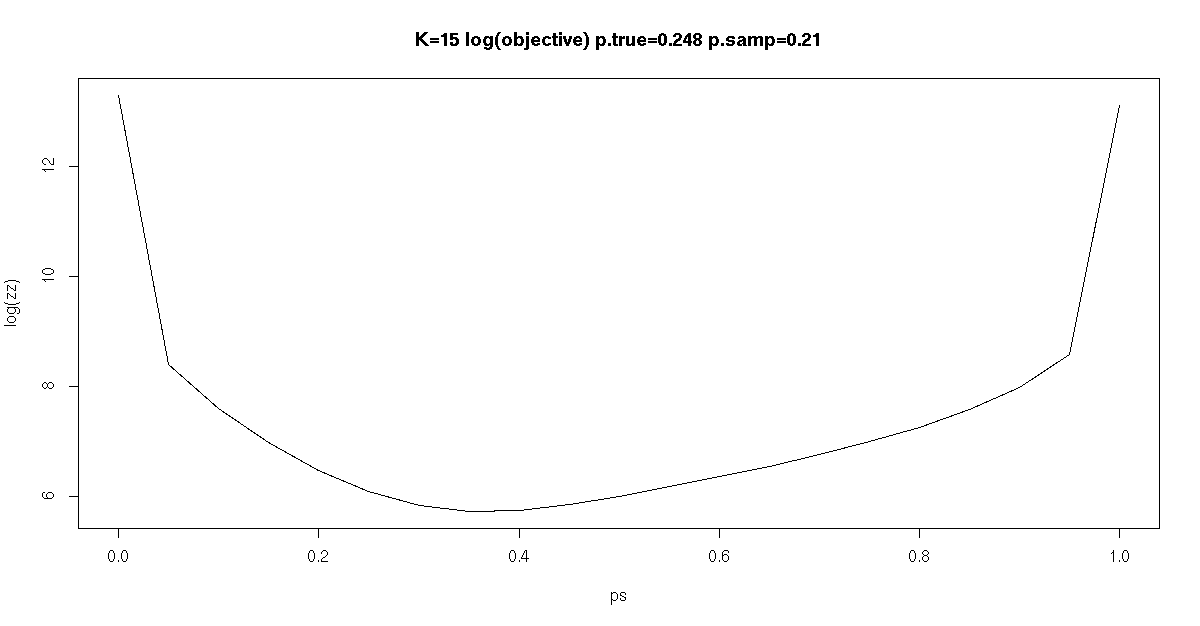
\includegraphics[scale=0.4]{log_obj_k15_q16.png}

This is interesting because Bernoulli model seems to prefer a higher $p$ estimate than sample frequency.


\end{document}
